\documentclass[11pt,a4paper]{article}

\usepackage{graphicx}
\usepackage[english]{babel}
\usepackage{authblk}
\usepackage{mathtools}
\DeclarePairedDelimiter{\ceil}{\lceil}{\rceil}
\usepackage{hyperref}
\hypersetup{
    colorlinks=true,       % false: boxed links, true: colored links
    linkcolor=black,       % color of internal links (change box color with linkbordercolor)
    citecolor=green,       % color of links to bibliography
    filecolor=magenta,     % color of file links
    urlcolor=blue          % color of external links
}

\setlength\parindent{0pt}                   % Fix indentation on new line
\setlength\parskip{\smallskipamount}
\frenchspacing

\renewcommand\Authand{, }

% The sweet relieve of a readable font.
\renewcommand{\familydefault}{\sfdefault}
\usepackage[T1]{fontenc}
\usepackage{amsmath}

\begin{document}

\title{Project artificial intelligence 2018-2019}
\author[1]{Olivier Van den Eede}
\author[1]{Dries Kennes}
\affil[1]{KU Leuven - De Nayer}
\date{}
\maketitle

\section{Problem Description}\label{sec:problem-description}
    The Cambio car sharing project lets you make a reservation for a car at a specific time in a specific zone.
    The goal of this optimization problem is to find the most optimal location for each car, in order to assign as many reservations as possible
    in one city.
    
    The city has been divided into zones, every car has a vehicle type and each reservation consists of:
    \begin{itemize} \itemsep-0.25em
        \item A required zone;
        \item A start and end date and time;
        \item A type of vehicle.
    \end{itemize} 

    This means a request can only be assigned to the required zone, or a neighboring zone.
    Only cars of the right type can be used for a reservation.
    And of-course a reservation can only be assigned if a car is free for the entire duration of the reservation.

    The goal is to assign each car to a zone, and assign each reservation to a car.
    No limit has been specified for the amount of cars assigned to one zone.

    The cost of this problem has to be as low as possible, and can be calculated by taking the sum of
    1) the $P$ factor if the request has not been assigned;
    and 2) the $Q$ factor if the request has been assigned to a neighbour
    as shown in formula~\ref{f:cost}.
    Every request has a different $P$ and $Q$ factor.

    \begin{equation}\label{f:cost}
        cost = \sum_{r}^{\#Requests} \left( P_r \cdot r_1 + Q_r \cdot r_2 \right)
    \end{equation}

    \begin{itemize} \itemsep-0.25em
        \item $r_1 = 1$ if $r$ is not assigned else $0$;
        \item $r_2 = 1$ if $r$ is assigned to a neighbour else $0$.
    \end{itemize}

\section{Our Solver}\label{sec:our-solver}

    We wrote our solver in Python 3, and will be using it's terminology in this paper.

    \subsection{Data Structures and Representation}\label{subsec:data-structures-and-representation}

        This is an overview of the data structures we use.

        \subsubsection{Request, Zone and Car}
            Requests and zones are parsed into objects of their respective class containing all fields necessary to store the input data in basic types.
            Cars do not have a custom object, they are represented with a simple string.

            After parsing the input data, all request and zone objects are stored in 2 lists, and in a dictionary each for fast lookup by id.
            These objects are all considered immutable so they never have to be copied.
        
        \subsubsection{Solution}
            A particular solution is represented by a Solution object.
            This object contains a reference to the parsed input data, and 2 dictionaries.
            These dictionaries represent the relationship between a car and zone, and between a request and a car.
            The cost function can be calculated based on the \texttt{car\_zone} and \texttt{req\_car} dictionaries.

            This is the only object that must be copied for every local move.
            This saves on memory churn and thus CPU time.

        \subsubsection{Overlap Matrix}
            To speed up some local moves, we pre-calculate a matrix of overlapping requests.
            This 2D boolean matrix allows for a fast feasibility check because the slow overlap checking loop is eliminated.


    \subsection{Algorithm}\label{subsec:algorithm}

        Our local search algorithm is composed of 3 major parts.

        \subsubsection{Greedy Assign}
            The greedy assign function loops over the currently unassigned requests, and tries to find a car already assigned to the right zone or a neighboring zone.
            If a suitable car is found, the request will be assigned.
            If no suitable car is available, the function will take a new car and assign it to the required zone and request.

            This function is used to create our initial solution, and guaranties a feasible solution.
            After each of our local moves, this function in called to try and fill all gaps and assign as many requests as possible.

        \subsubsection{Local Moves}
            Our algorithm is based around 5 small local changes:
            \begin{itemize} \itemsep-0.25em
                \item Move a request from the 'optimal' zone to one of its neighbors
                \item Move a request assigned to a neighbor zone to the 'optimal' zone.
                \item Swap the car assigned to a request with another car in the same zone.
                \item Unassign 1 car from all its requests.$^\dagger$
                \item Unassign 1 request.$^\dagger$
            \end{itemize}
            The local moves with \textdagger~are twice as likely to be chosen.
            This multiplier has been imperially determined.

            None of these moves make the solution infeasible.
            This potentially limits the search space that can be reached, but it also make the computation less complex and thus much faster.

        \subsubsection{Metaheuristic}\label{subsec:metaheuristic}
            To control all small local changes, we implemented simulated annealing.
            This allows our algorithm to find a different solution in the neighborhood of the working solution.
            This new solution will be accepted if the cost is lower, and accepted or rejected with a random probability based on the simulated annealing factors.
            When the stop-condition for our algorithm is reached, a new random initial solution will be generated and start again.

            Our parameters:
            \begin{itemize} \itemsep-0.25em
                \item $T_{\max} = 1000$;
                \item $T_{\min} = 10$;
                \item $\alpha = 0.65$;
                \item $N = 5000$.
            \end{itemize}
            This results in $5000\ceil{\log_{0.65}(1000/10)} = 55000$ iterations per completed run.

            The data we used to justify our simulated annealing parameters can be found in the attached archive, or online on
            \href{https://cambio.dries007.net/sa_parameter_tests/}{\texttt{cambio.dries007.net/sa\_parameter\_tests}}.

    \subsection{Determinism}\label{subsec:determinism}
        Despite our best efforts our solver is not deterministic, i.e., the same seed input does not result in the same output.
        We are not sure why that is the case, but decided it was not worth spending more time on.


\section{Results}\label{sec:results}

    We consider our implementation a success.
    We reach results at least 10\% better than the published results on Toledo with the 300 seconds on 2 threads.
    The results in table~\ref{tab:results} results are the median of a number of runs.
    Figure~\ref{fig:graph} is a separate run because the data to generate the graphs is not saved on normal runs.
    Every line on the graph is one iteration of the simulated annealing part.

    \begin{table}[ht]
        \centering
        \begin{tabular}{r|r|r|r}
            Bestand                     & Toledo  & Score & Improvement \\\hline
            \texttt{100\_5\_14\_25.csv} &  10015  &  8795 &    12.18\%  \\
            \texttt{100\_5\_19\_25.csv} &   6700  &  6045 &     9.78\%  \\
            \texttt{210\_5\_33\_25.csv} &  14325  & 11180 &    21.95\%  \\
            \texttt{210\_5\_44\_25.csv} &   5890  &  4045 &    31.32\%  \\
            \texttt{360\_5\_71\_25.csv} &  12955  &  7490 &    42.18\%  \\
        \end{tabular}
        \caption{Our results compared to the scores on Toledo.}
        \label{tab:results}
    \end{table}

    \subsection{Performance}\label{subsec:performance}
        Our solver manages to perform in the order of 12000 local moves per second (or 12kHz) with an input of 100 requests on an Intel i5-4670 CPU running at 4GHz.
        For the 210 requests example file we reach 10kHz. With 360 requests the performance is 5KHz.

        This performance is reached thanks careful analysis of the code and runtime profiling.
        Removal of unused sections of the algorithm such as the feasibility check (since we never make a solution non feasible), made a very considerable (up to 50\%) difference.
        List creations have been replaced with generators wherever possible.
        Short circuiting also helps reduce the average time spent checking overlap for example.
        The solution object is only cloned if it has to be, meaning if a local move failed, it can be used again for the next attempt.

        With our simulated annealing parameters as mentioned in~\ref{subsec:metaheuristic}, the time for a single iteration of our algorithm remains low (order of ten seconds).
        This means that we can run many iterations in the given time limit (5 minutes).
        This creates many opportunities to find a good solution, even if our algorithm cannot reach all of the solution space.

    \subsection{Search Space}\label{subsec:search-space}
        Because our algorithm uses \textit{Greedy Assign} after every successful local move, it cannot reach all of the search space.
        For example: We cannot unassign two cars without attempting to assigning requests to them.
        We consider this a downside of our implementation.

    \subsection{Possible Improvements}\label{subsec:possible-improvements}
        We consider the following items possible improvements, or at least worthy of future research:
        \begin{itemize} \itemsep-0.25em
            \item Attempting to reach more of the search space, as mentioned in~\ref{subsec:search-space}.
            \item Adding more local moves.
            \item Researching the chance multipliers the local moves use.
            \item Allowing the solution to become infeasible, to reach disjointed regions in the search space.
        \end{itemize}


\pagebreak\section{Appendix}\label{sec:appendix}

\begin{figure}[ht]
    \centering
    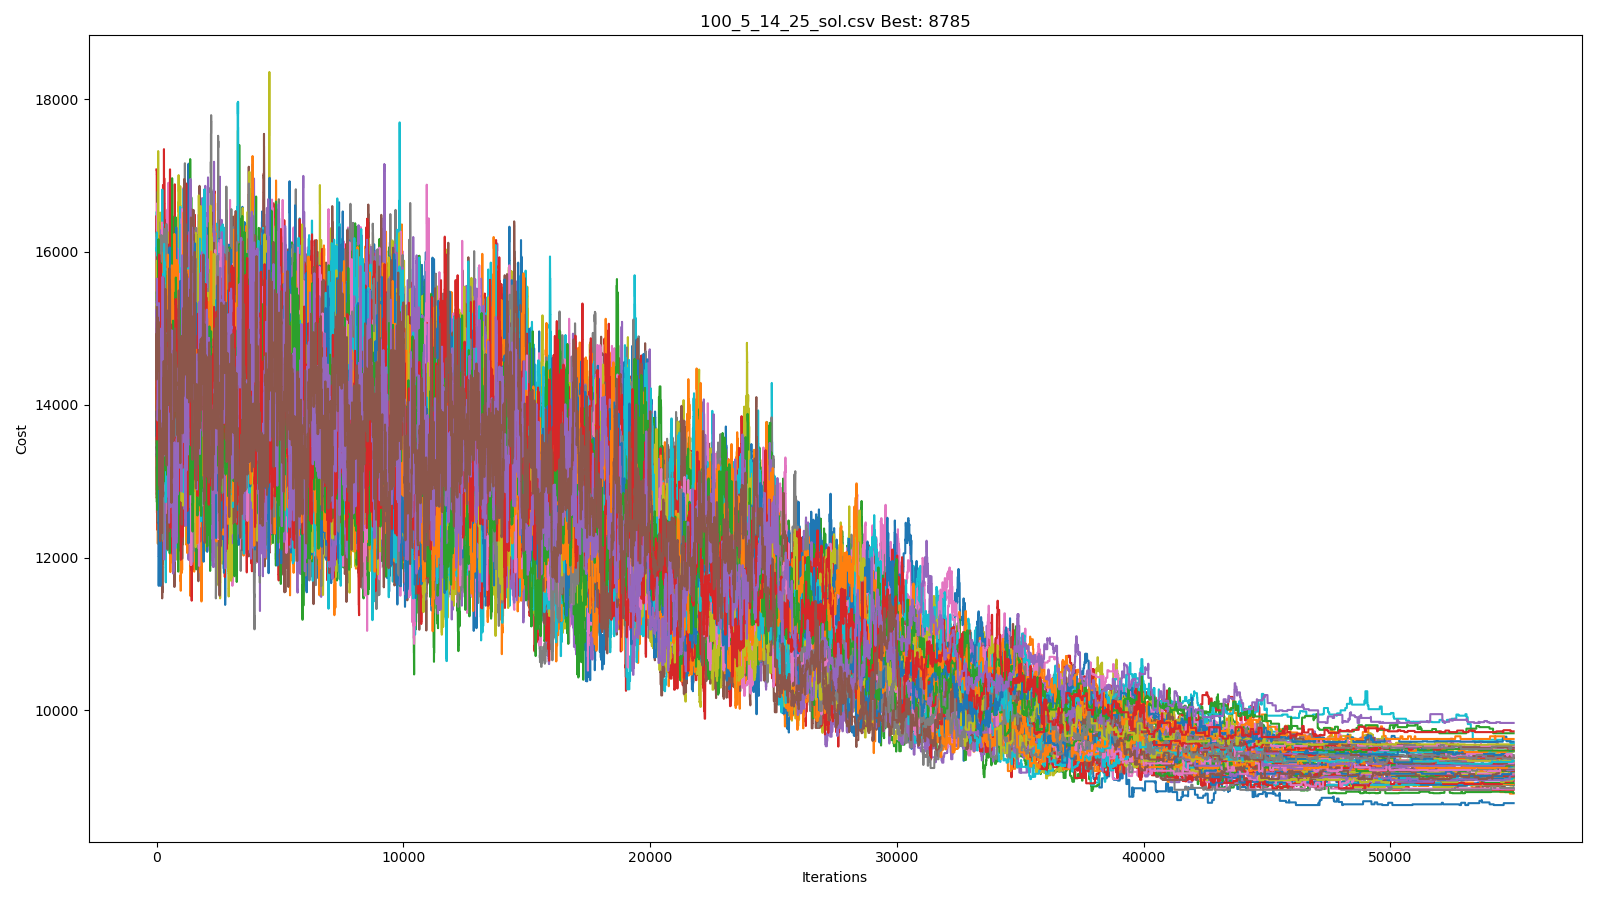
\includegraphics[width=\textwidth]{../img/100_5_14_25.png}
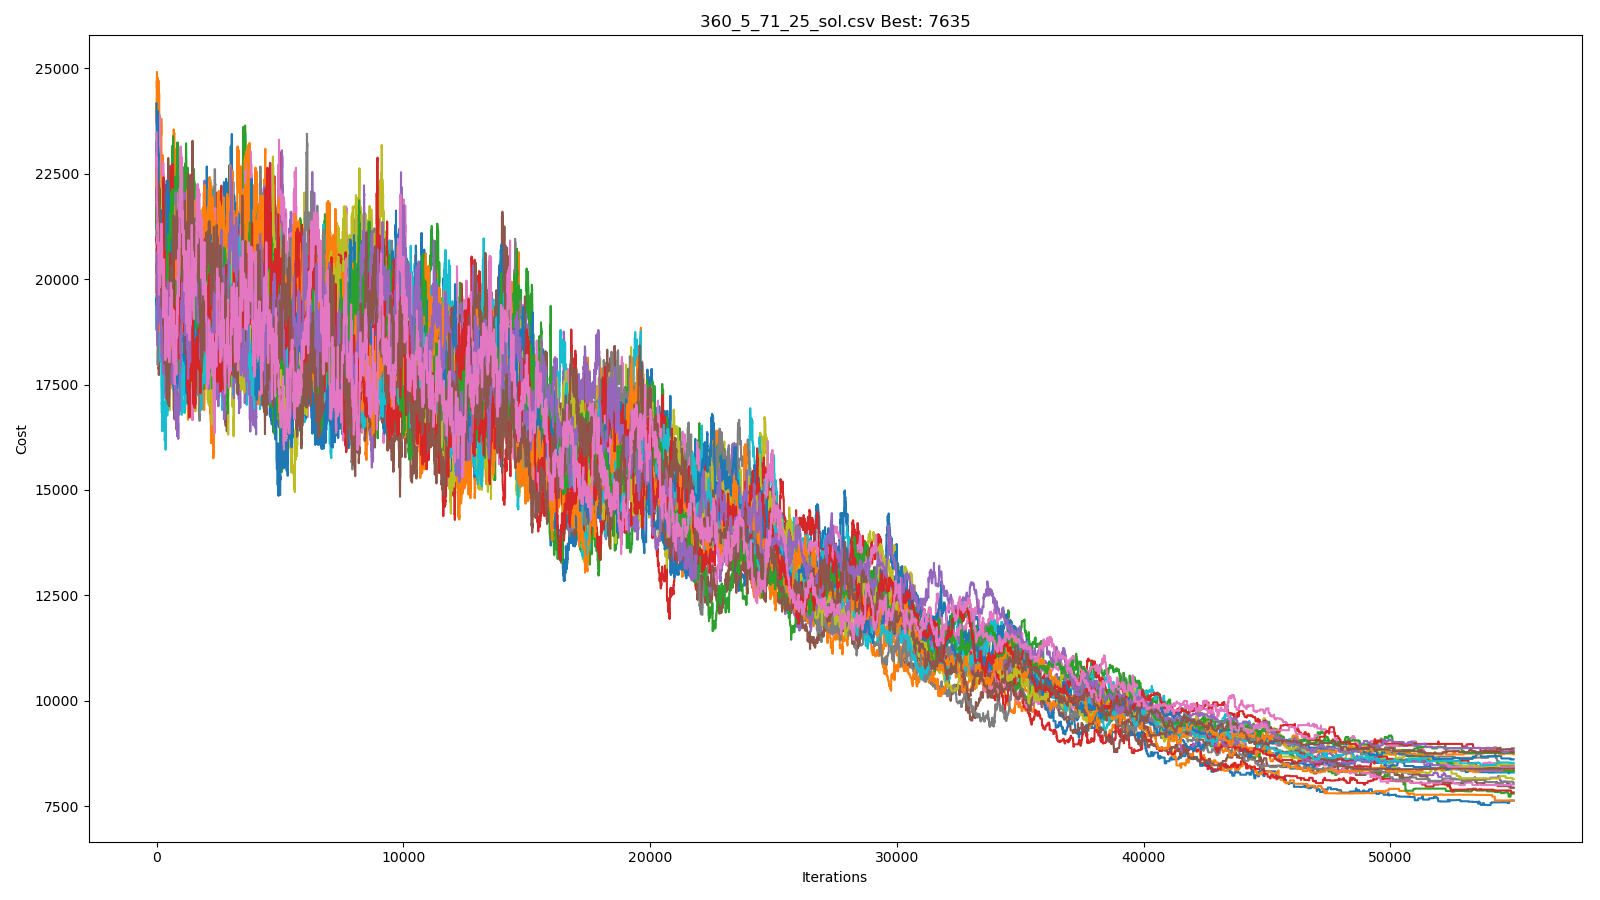
\includegraphics[width=\textwidth]{../img/360_5_71_25.png}
    \caption{Debug run of \texttt{100\_5\_14\_25.csv} and \texttt{360\_5\_71\_25.csv}.
             These images are also hosted on \href{https://cambio.dries007.net/img/}{\texttt{cambio.dries007.net/img}}.}
    \label{fig:graph}
\end{figure}


\end{document}